\chapter{Problema de estimación de sexo}
\label{chap:sex_estimation}

Se propone un problema adicional, para la estimación de sexo a partir de los imágenes de las radiografías maxilofaciales. Para este problema de clasificación binaria identificamos dos clases: sexo masculino (M) y sexo femenino (F).

% ¿Qué esperamos que haga?


En la Tabla \ref{tab:SE-accuracy_EC_MPSS} se recogen las métricas obtenidas por los diferentes métodos. La exactitud apenas se reduce en medio punto porcentual entre los métodos conformales y el método `base', en la línea de resultados infímamente peores en los primeros.

Por otro lado, la cobertura del método `base', al solo incluir la etiqueta de la clase más probable en el conjunto de predicción, presenta una cobertura empírica igual a la exactitud, del 88.57\%. LAC y MCM sí logran una cobertura del 95\%, con un 18\% de las instancias indeterminadas (con ambas etiquetas en el conjunto de predicción) en promedio, en ambos casos. Finalmente, en la gráfica de dispersión de la Figura \ref{fig:SE-scatterplot_EC_MPSS} se observa que no existen diferencias relevantes entre los métodos conformales, cuyos resultados se solapan en el diagrama.

\renewcommand{\arraystretch}{1.4}
\begin{table}[h]
    \small
    \centering
    \begin{tabular}{cccclccccccc}
    \toprule
    \multirow{2}{*}{\textbf{Método}} &  & \multicolumn{2}{c}{\textbf{Exactitud (\%)}} &  & \multicolumn{3}{c}{\textbf{\begin{tabular}[c]{@{}c@{}}Cobertura\\[-0.8ex] Empírica (\%)\end{tabular}}} &  & \multicolumn{3}{c}{\textbf{\begin{tabular}[c]{@{}c@{}}Tamaño Medio\\[-0.8ex] del Conjunto\end{tabular}}} \\ 
    \cline{3-4} \cline{6-8} \cline{10-12} 
    &  & \textbf{base} & \textbf{CP} &  & \textbf{base} & \textbf{LAC} & \textbf{MCM} &  & \textbf{base} & \textbf{LAC} & \textbf{MCM} \\ 
    \cline{1-1} \cline{3-4} \cline{6-8} \cline{10-12} 
    Ejecución 1 &  & 88.75 & 87.04 &  & 88.75 & 94.19 & 94.33 &  & 1.00 & 1.18 & 1.19 \\
    Ejecución 2 &  & 89.08 & 89.03 &  & 89.08 & 96.24 & 96.42 &  & 1.00 & 1.20 & 1.21 \\
    Ejecución 3 &  & 89.64 & 88.15 &  & 89.64 & 94.98 & 94.56 &  & 1.00 & 1.16 & 1.15 \\
    Ejecución 4 &  & 88.10 & 88.75 &  & 88.10 & 94.84 & 94.89 &  & 1.00 & 1.17 & 1.15 \\
    Ejecución 5 &  & 88.20 & 88.29 &  & 88.20 & 95.91 & 95.68 &  & 1.00 & 1.20 & 1.17 \\
    Ejecución 6 &  & 88.48 & 87.04 &  & 88.48 & 94.75 & 94.93 &  & 1.00 & 1.19 & 1.19 \\
    Ejecución 7 &  & 88.80 & 86.99 &  & 88.80 & 95.03 & 94.56 &  & 1.00 & 1.22 & 1.21 \\
    Ejecución 8 &  & 87.50 & 87.83 &  & 87.50 & 94.89 & 95.12 &  & 1.00 & 1.17 & 1.17 \\
    Ejecución 9 &  & 88.94 & 88.48 &  & 88.94 & 94.70 & 94.89 &  & 1.00 & 1.15 & 1.14 \\
    Ejecución 10 &  & 88.20 & 88.57 &  & 88.20 & 95.77 & 94.80 &  & 1.00 & 1.21 & 1.17 \\ 
    \cline{1-1} \cline{3-4} \cline{6-8} \cline{10-12} 
    Media &  & \textbf{88.57} & 88.02 &  & 88.57 & \textbf{95.13} & \textbf{95.02} &  & 1.00 & \textbf{1.18} & \textbf{1.18} \\ 
    \bottomrule
    \end{tabular}
    \caption[
        Problema de estimación de mayoría de sexo: 
        Valores de exactitud, cobertura empírica y tamaño medio del conjunto obtenidas por cada método de predicción a lo largo de 10 ejecuciones.
    ]{
        Valores de exactitud, cobertura empírica y tamaño medio del conjunto obtenidas por cada método de predicción a lo largo de 10 ejecuciones, así como la media final para cada método entre todas las ejecuciones. 
        `CP' se refiere a los métodos conformales empleados: LAC y MCM (se recuerda que es el mismo modelo para todos los métodos conformales y, por ello, presentan los mismas predicciones puntuales). 
        Se marca en negrita las medias con mejor marca para cada métrica: mayor valor en exactitud, valores próximos a 95\% en cobertura empírica y mínimo valor en tamaño medio del conjunto.
    }
    \label{tab:SE-accuracy_EC_MPSS}
\end{table}


\begin{figure}[h]
    \centering
    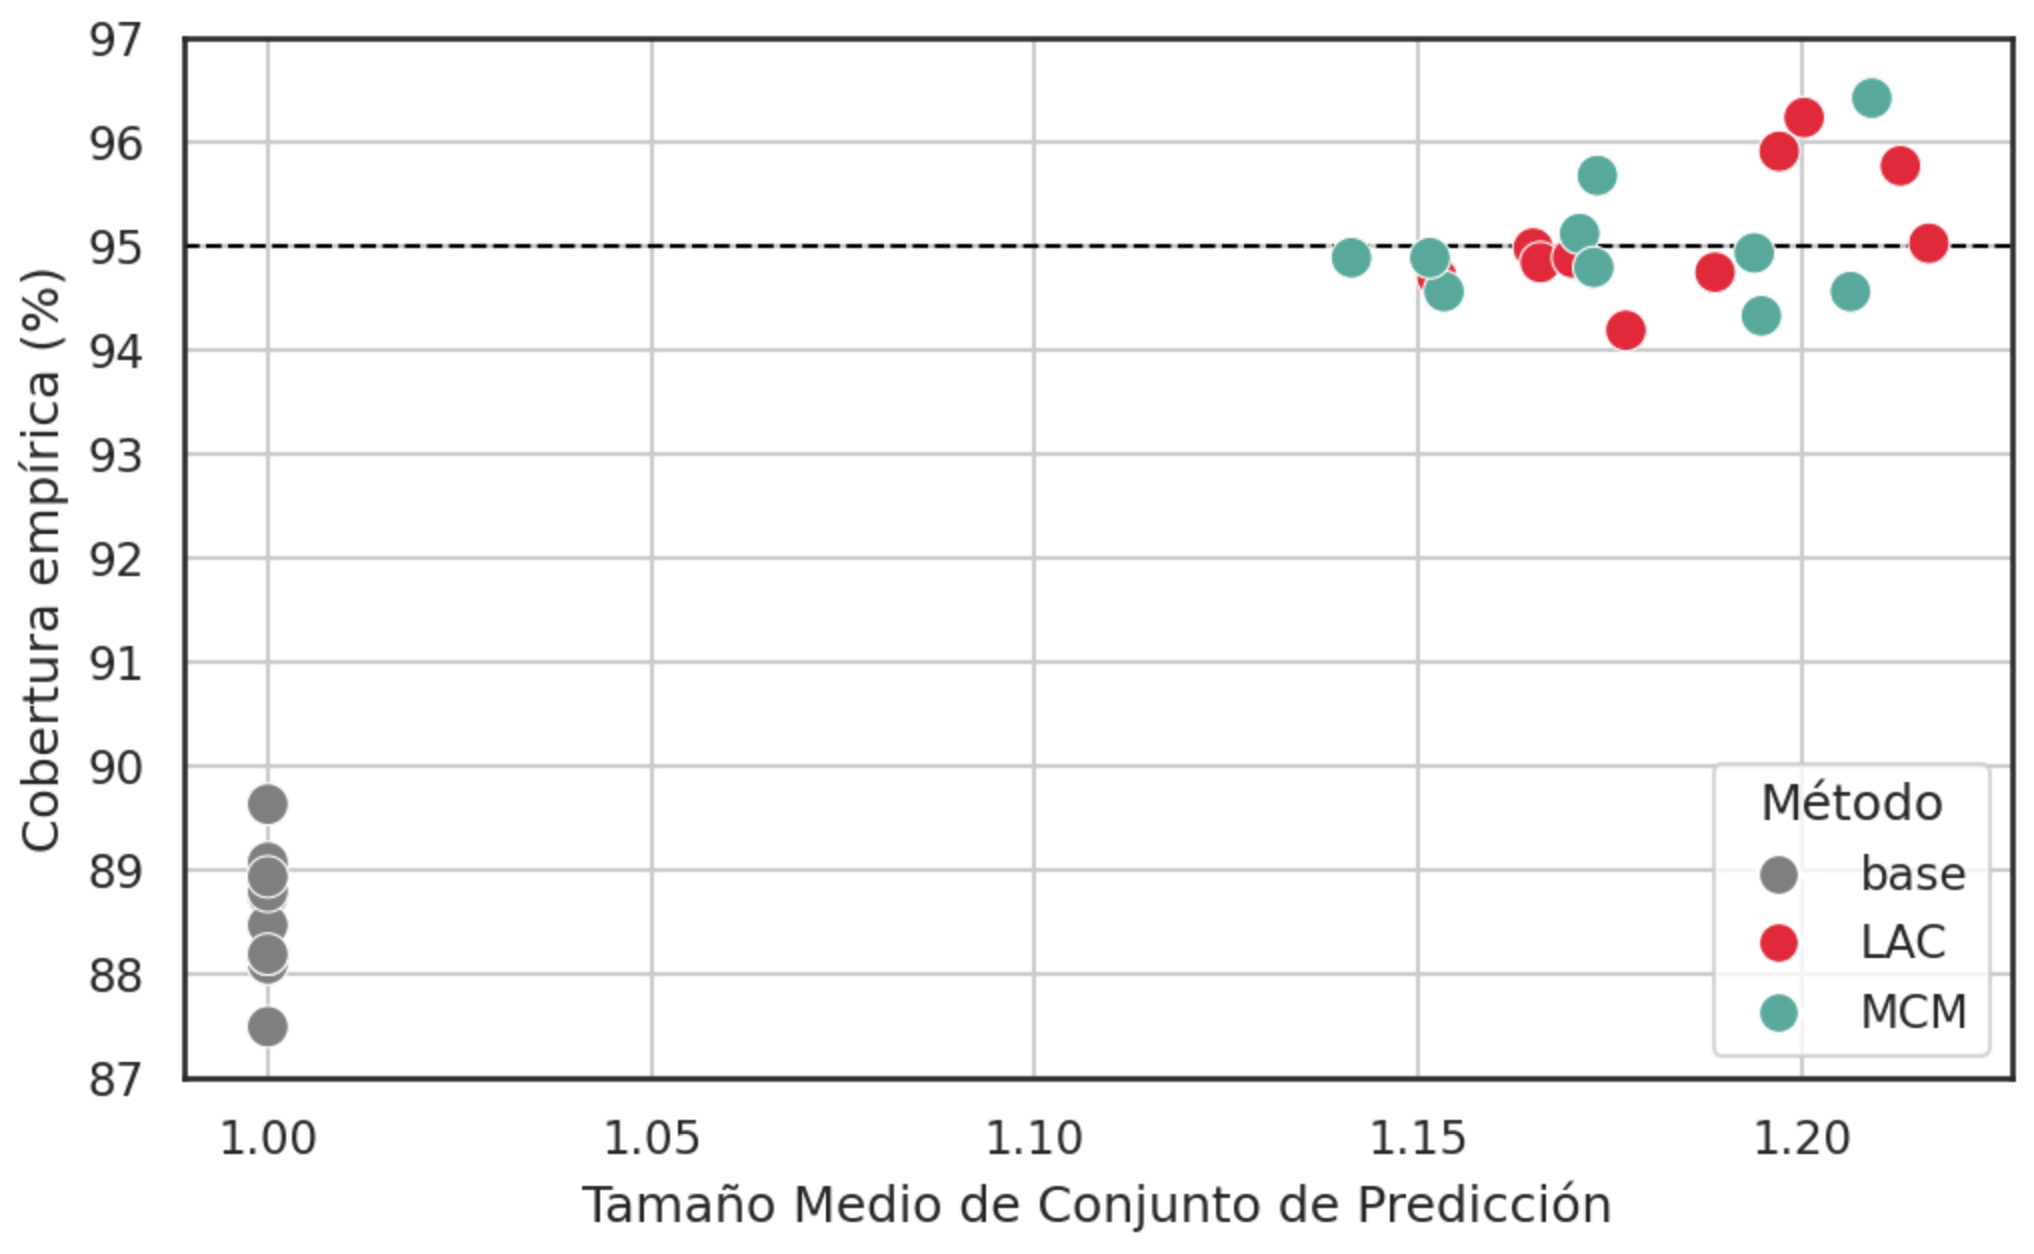
\includegraphics[width=0.9\textwidth]{apendices/imagenes/SE-scatterplot_EC_MPSS.png}
    \caption[
        Problema de estimación de sexo: 
        Gráfica de dispersión de la cobertura empírica frente al tamaño medio de conjunto de predicción.
    ]{
        Gráfica de dispersión de la cobertura empírica frente al tamaño medio de conjunto de predicción.
    }
    \label{fig:SE-scatterplot_EC_MPSS}
\end{figure}



A continuación, en la Figura \ref{fig:SE-heatmap_EC_by_PSS} se analiza la cobertura en función del tamaño del conjunto. Se observa que aproximadamente un 18\% de las instancias presenta un conjunto de predicción indeterminado, el cual, como es obvio, alcanza una cobertura del 100\%. El 82\% restante de las instancias obtiene una cobertura cercana al 94\%, tanto con el método LAC como con MCM.


\begin{figure}[h]
    \centering
    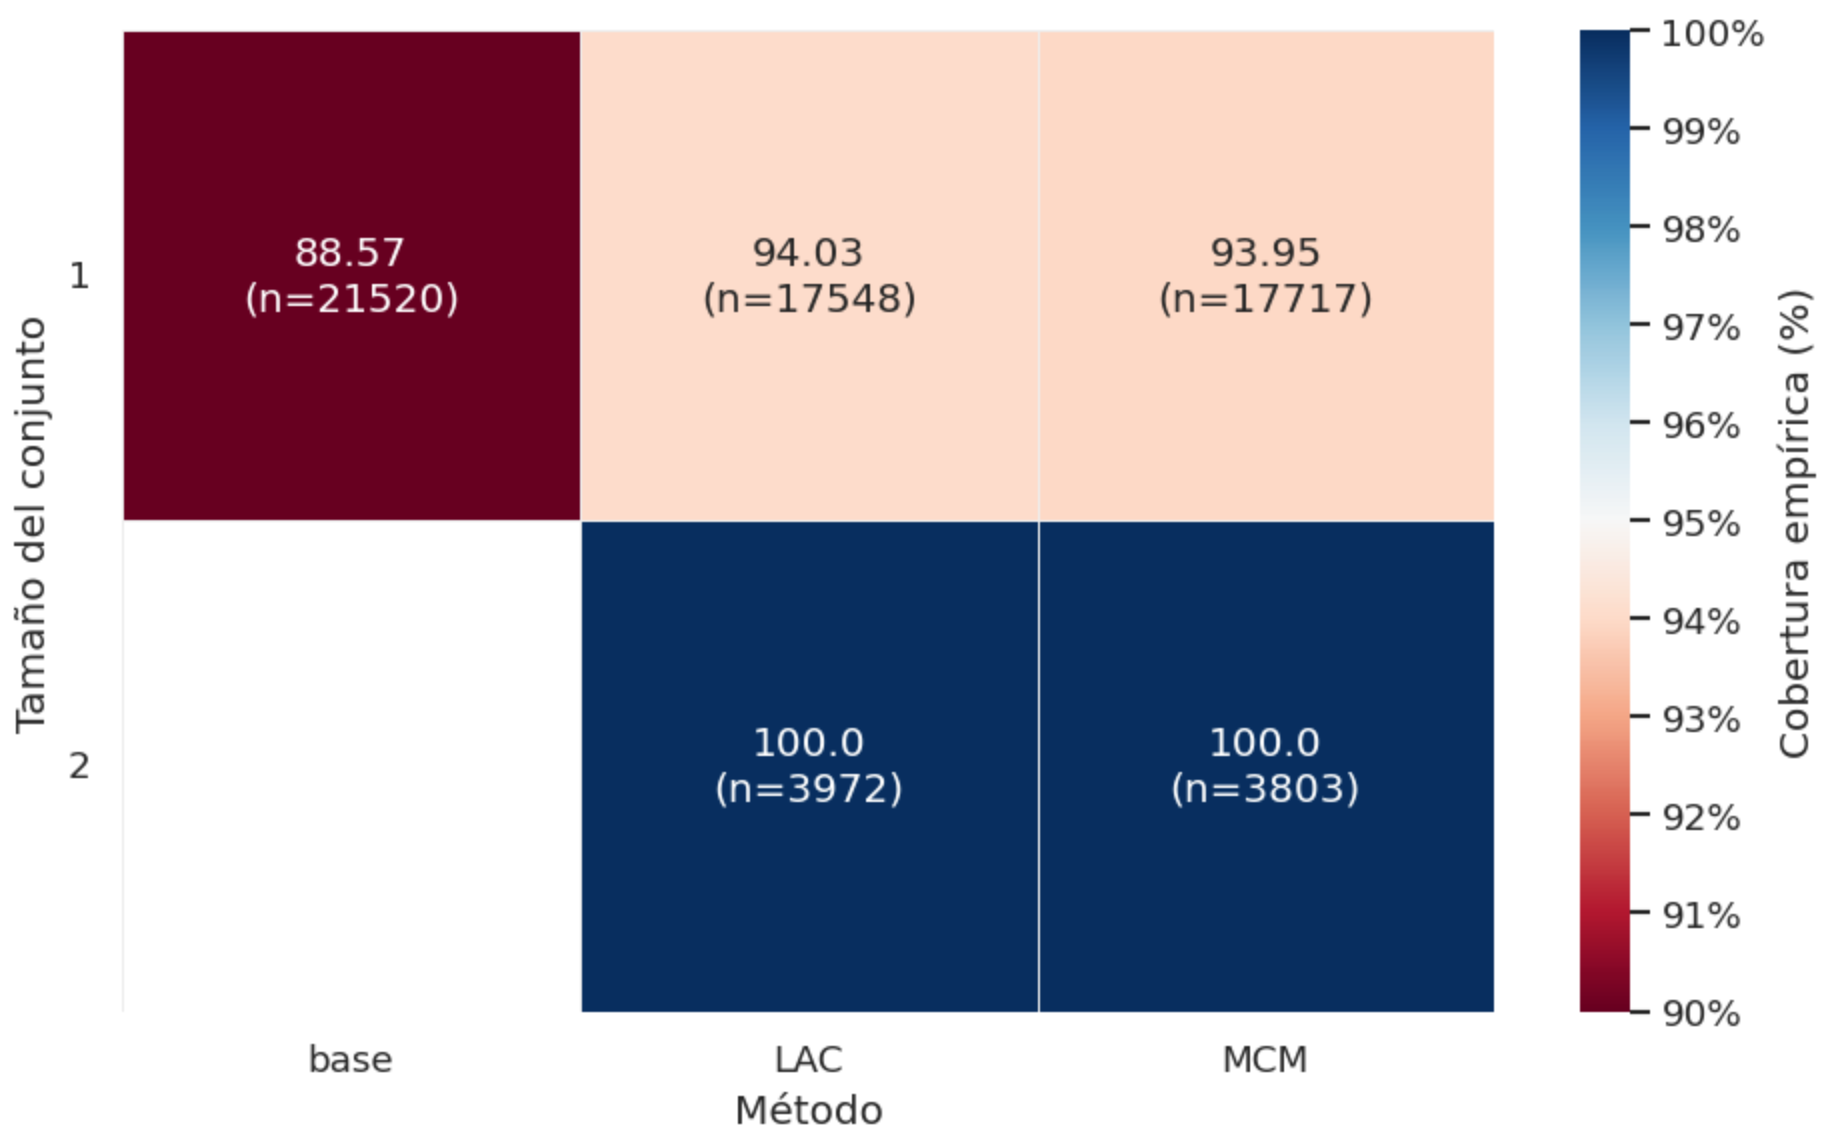
\includegraphics[width=0.9\textwidth]{apendices/imagenes/SE-heatmap_EC_by_PSS.png}
    \caption[
        Problema de estimación de sexo: 
        Mapa de calor de la cobertura empírica en base al tamaño del conjunto por cada método de predicción a lo largo de 10 ejecuciones.
    ]{
        Mapa de calor de la cobertura empírica en base al tamaño del conjunto por cada método de predicción a lo largo de 10 ejecuciones.
        Se especifica entre paréntesis el número de instancias con el número de etiquetas en el conjunto de predicción.
        La escala de colores está centrada en la cobertura nominal ($0.95$): los valores por debajo de este umbral se representan en tonos rojos, los superiores en tonos azules, y el blanco indica una cobertura empírica equivalente a la nominal.
    }
    \label{fig:SE-heatmap_EC_by_PSS}
\end{figure}

En definitiva, el método `base' logra: 88.57\% de las instancias bien clasificadas, y el 11.43\% mal clasificadas. Frente a esto, los métodos conformales logran: 77\% de las intancias bien clasificadas, 5\% mal clasificadas, y un 18\% indeterminadas (véase la Figura \ref{fig:SE-outputs_comparative}). De esta forma, se ha conseguido reducir la proporción de instancias mal clasificadas de un 11.43\% a un 5\%, aunque a cambio se generan instancias indeterminadas que, en el método base, habrían sido clasificadas correctamente.

\begin{figure}[h]
    \centering
    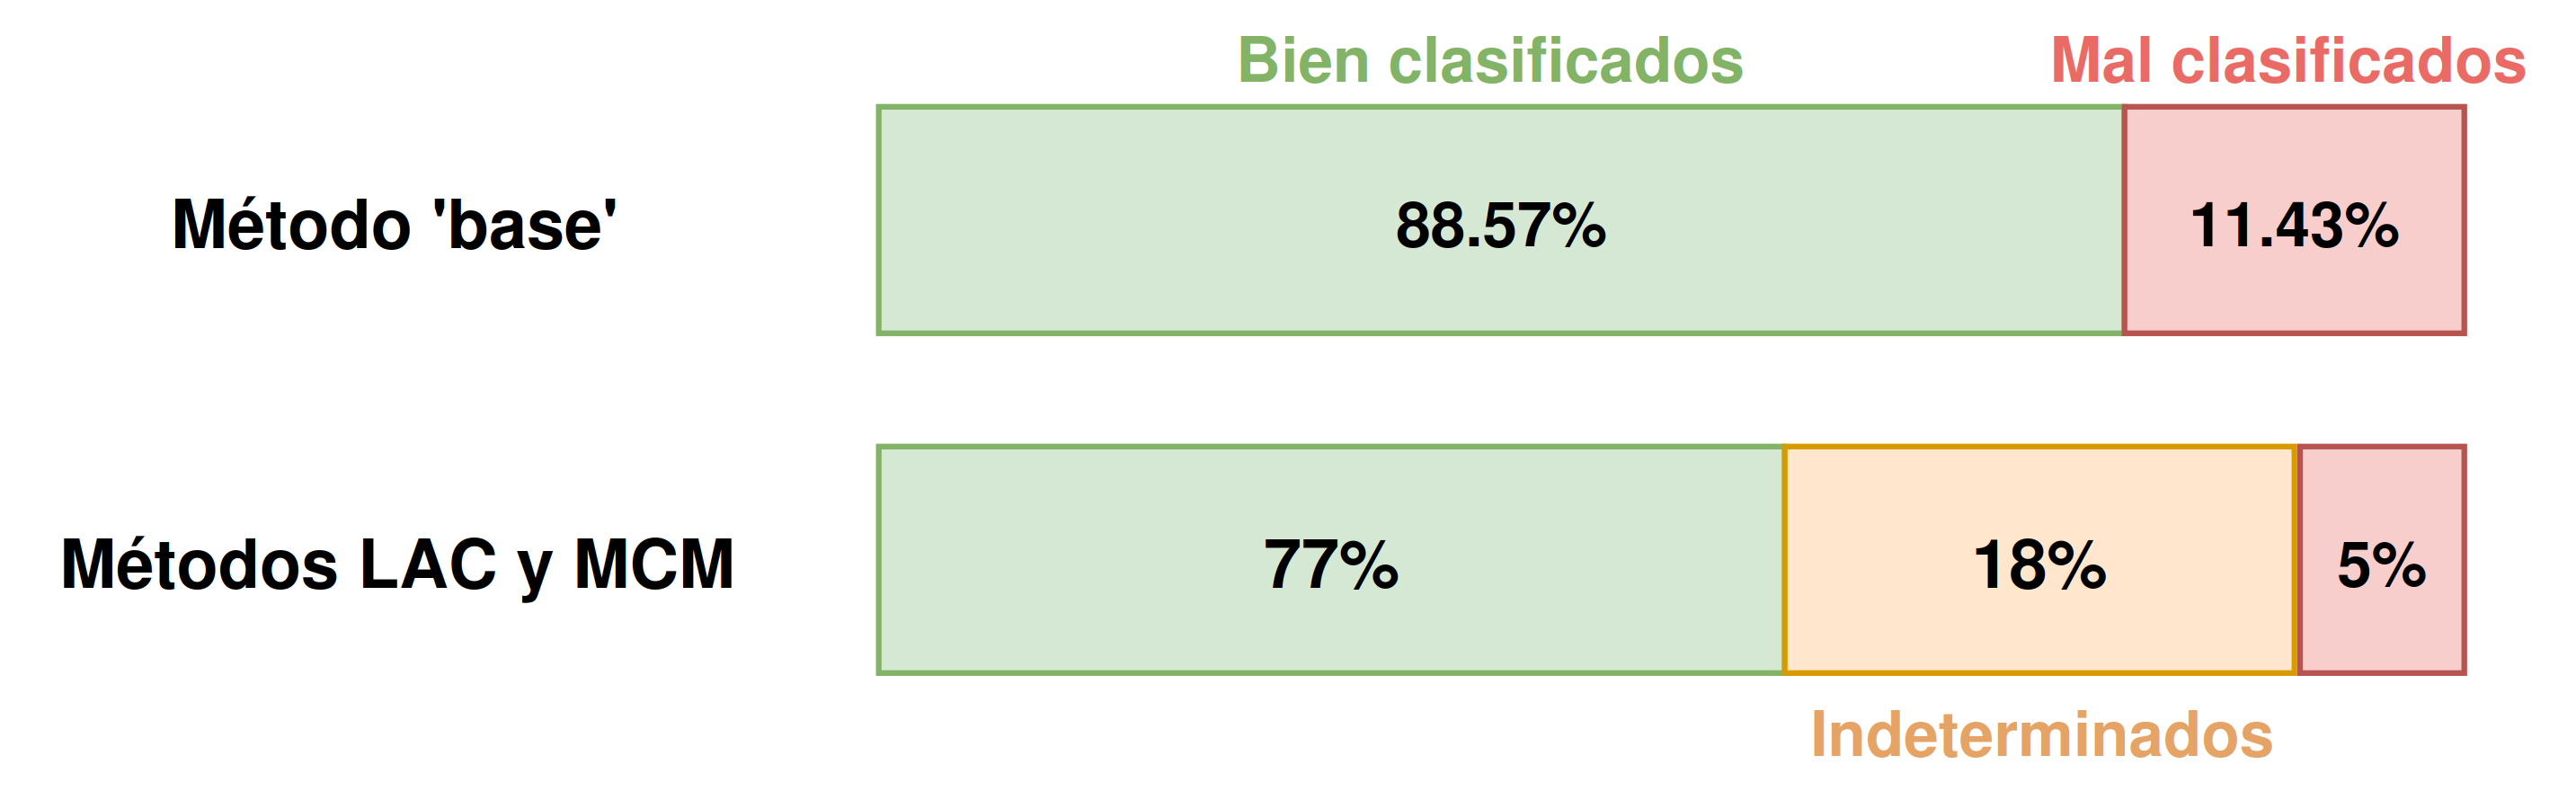
\includegraphics[width=0.9\textwidth]{apendices/imagenes/SE-outputs_comparative.png}
    \caption[
        Problema de estimación de sexo: 
        Proporción de instancias bien clasificadas, mal clasificadas e indeterminadas de los métodos propuestos.
    ]{
        Proporción de instancias bien clasificadas, mal clasificadas e indeterminadas de los métodos propuestos.
    }
    \label{fig:SE-outputs_comparative}
\end{figure}

Y, por último, vamos a analizar la cobertura en base al sexo y la edad, a partir de las Figuras \ref{fig:SE-linechart_EC_by_age_and_sex} y \ref{fig:SE-linechart_MPSS_by_age_and_sex}. Se pueden observar varias tendencias en el método `base':

\begin{itemize}
    \item Se dan más errores de clasificación en las edades más jóvenes que en las avanzadas, de lo que se puede inferir que existe mayor incertidumbre en edades jóvenes. Probablemente este efecto sea consecuencia de que los rasgos sexuales maxilofaciales aún no están lo suficientemente marcados en edades jóvenes.
    
    \item Hay más instancias mal clasificadas en varones que en hembras, para prácticamente todas las edades. Esto indica que también existe mayor incertidumbre en individuos de sexo masculino, debido a que el desarrollo de caracteres sexuales secundarios faciales se complta más tardíamente que en las hembras.

\end{itemize}

No obstante, estas dos fuentes de incertidumbre son abordadas por los métodos LAC y MCM mediante el uso de conjuntos indeterminados, los cuales permiten representar de forma explícita la ambigüedad en la clasificación. De este modo, la cobertura alcanzada por ambos métodos supera el 90\% en prácticamente todas las edades y sexos, y en la mayoría de las combinaciones sexo-edad llega incluso a aproximar o superar el 95\%, manteniendo ---aunque en menor medida--- las tendencias descritas anteriormente.


\begin{figure}[h]
    \centering
    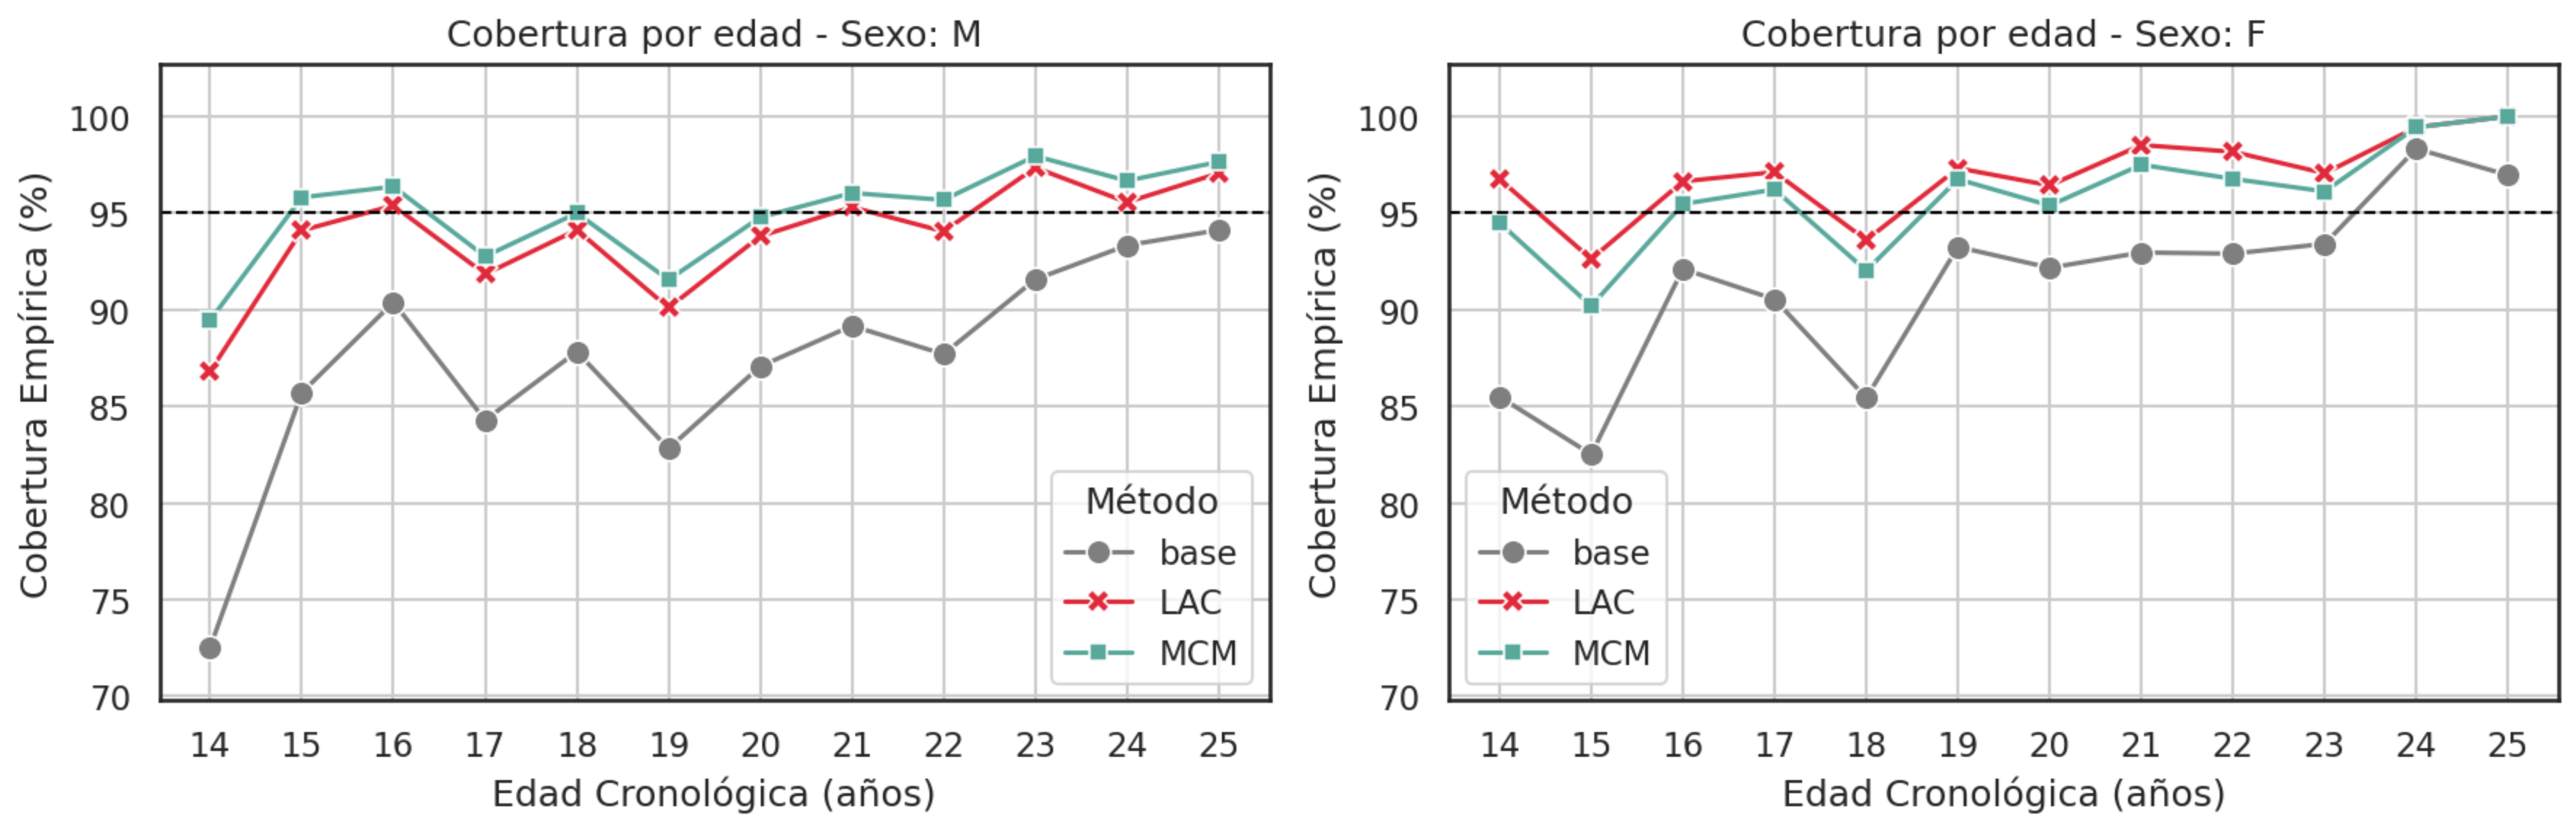
\includegraphics[width=\textwidth]{apendices/imagenes/SE-linechart_EC_by_age_and_sex.png}
    \caption[
        Problema de estimación de sexo:
        Diagrama de líneas de la cobertura empírica en base al sexo y la edad cronológica por cada método de predicción a lo largo de 10 ejecuciones.
    ]{
        Diagrama de líneas de la cobertura empírica en base al sexo y la edad cronológica por cada método de predicción a lo largo de 10 ejecuciones.
    }
    \label{fig:SE-linechart_EC_by_age_and_sex}
\end{figure}


\begin{figure}[h]
    \centering
    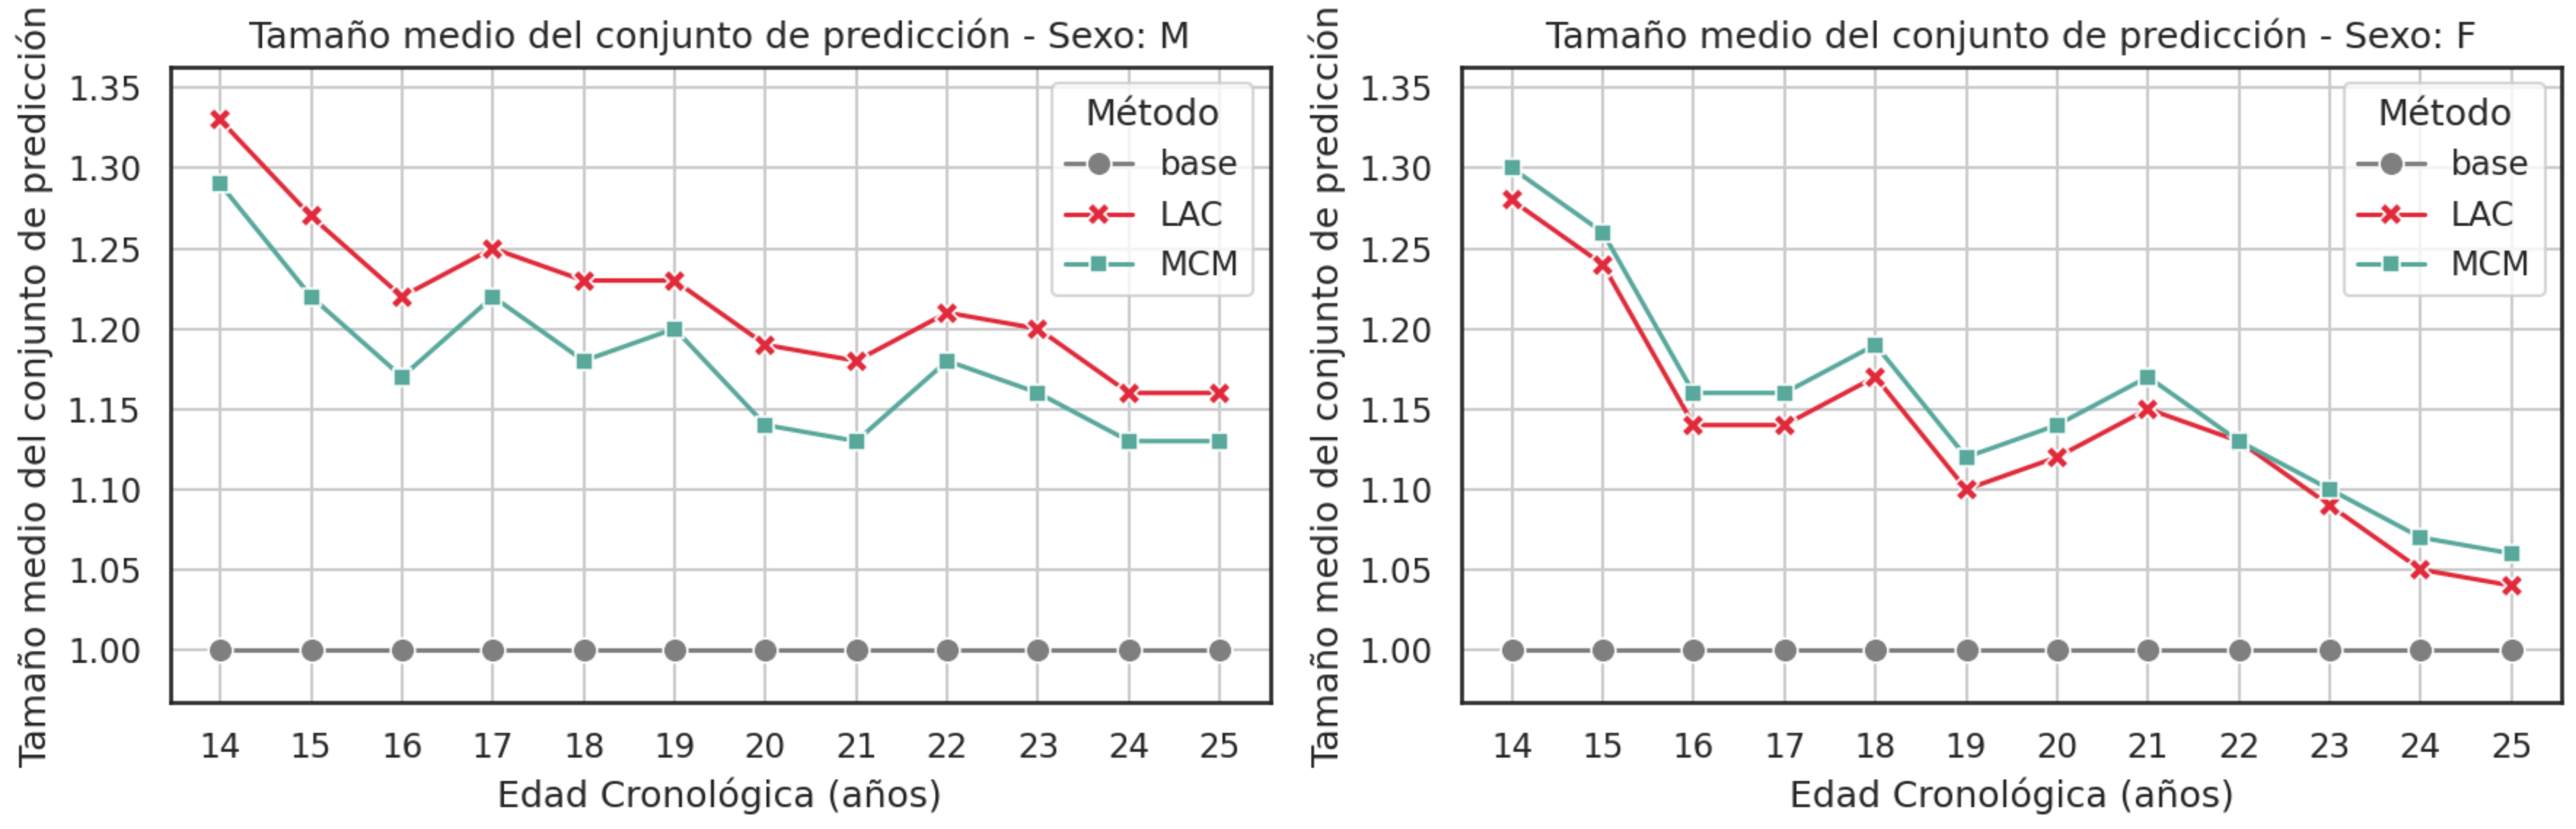
\includegraphics[width=\textwidth]{apendices/imagenes/SE-linechart_MPSS_by_age_and_sex.png}
    \caption[
        Problema de estimación de sexo:
        Diagrama de líneas del tamaño medio de conjunto de predicción en base al sexo y la edad cronológica por cada método de predicción a lo largo de 10 ejecuciones.
    ]{
        Diagrama de líneas del tamaño medio de conjunto de predicción en base al sexo y la edad cronológica por cada método de predicción a lo largo de 10 ejecuciones.
    }
    \label{fig:SE-linechart_MPSS_by_age_and_sex}
\end{figure}

